\subsection*{Цель работы}

\begin{enumerate}
    \item Изучение цикловой СУ ЭЦПУ-6030.
    \item Изучение промышленных роботов МП-9, МП-11 и 202М.
\end{enumerate}

\subsection*{Общие сведения}

ЭЦПУ-6030 может работать в следующих режимах:

\begin{itemize}
    \item автоматическом;
    \item покадровом;
    \item ручном.
\end{itemize}

СУ работает по принципу структурно-алгоритмической организации. Структурная схема ЭЦПУ 6030 показана на рисунке \ref{fig:structure60}.

ЭЦПУ-6030 может работать:

\begin{itemize}
    \item команда --- выполнение одной команды;
    \item цикл --- отработка всех команд с наборного поля за один цикл;
    \item автоматический --- многократная отработка кадров программы.
\end{itemize}

\begin{figure}[ht]
    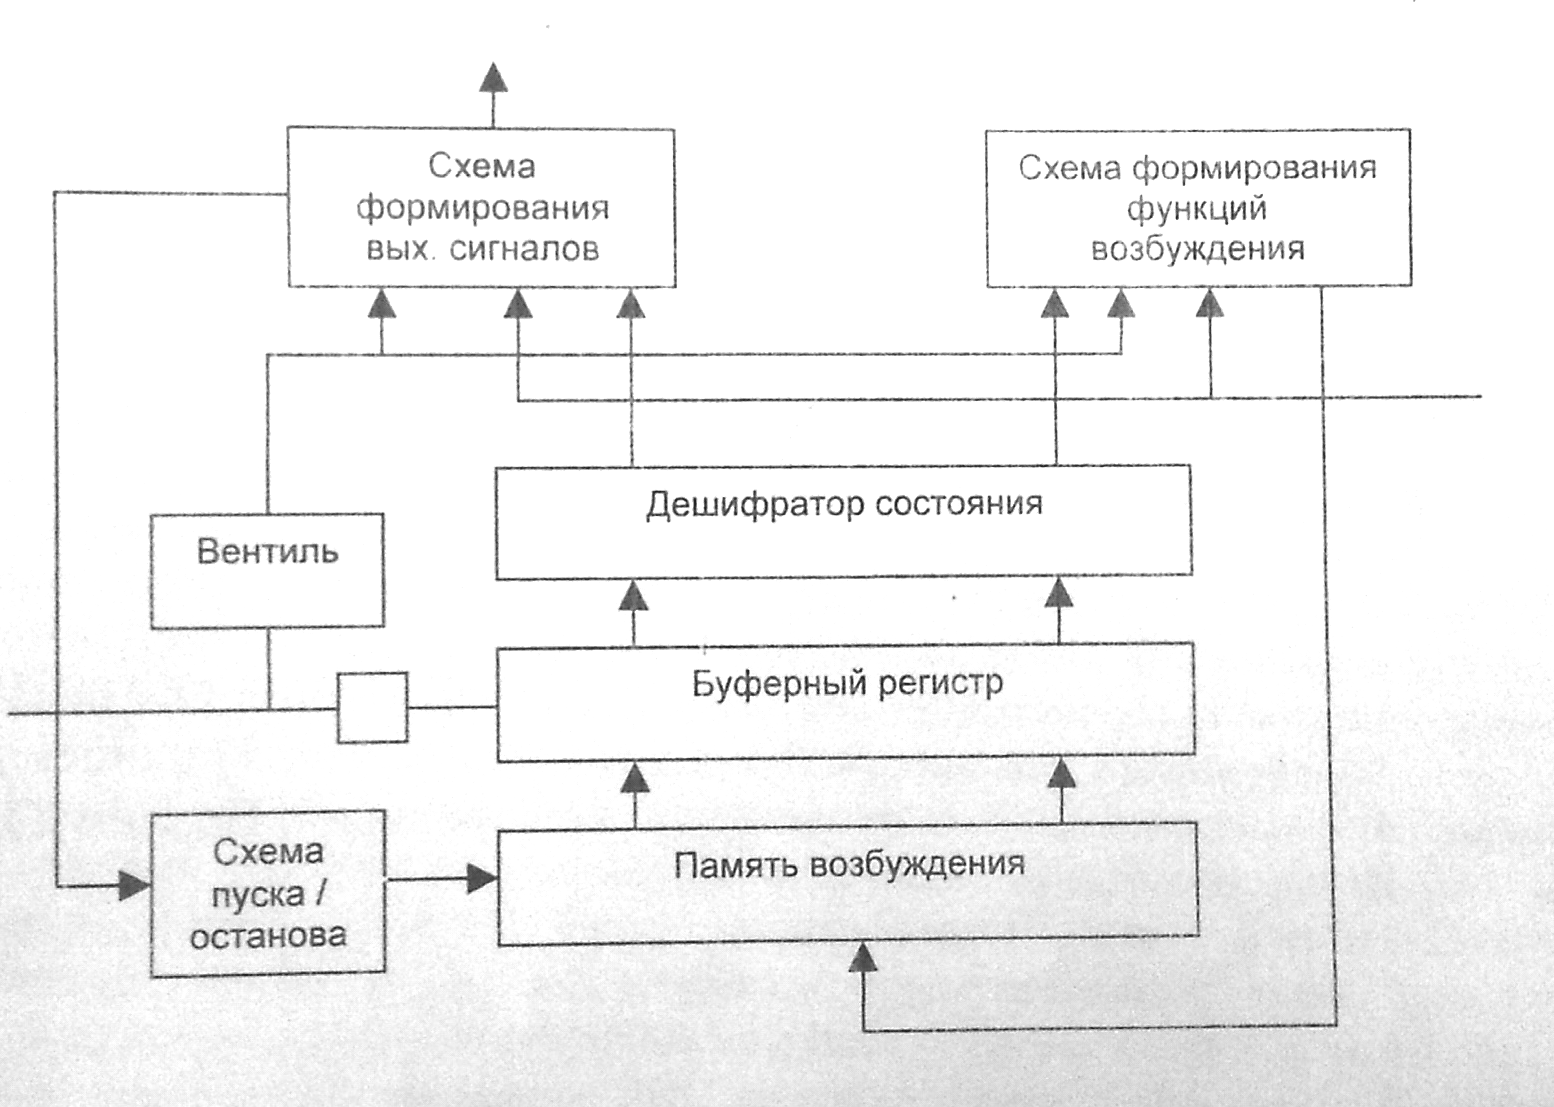
\includegraphics[width=1\linewidth]{Figures/structure60.png}
    \caption{Структурная схема ЭЦПУ 6030}
    \label{fig:structure60}
\end{figure}

Основной принцип циклового управления автоматическими роботами, заключающийся в осуществлении позиционирования манипулятора по упорам, определяет ряд характерных особенностей цикловых систем управления, главными из которых являются следующие:

\begin{itemize}
    \item программирование логической и технологической информации дискретного вида, определяющей последовательность движения звеньев манипулятора, длительность позиционирования;
    \item выделение информации о перемещениях по отдельным степеням подвижности, задаваемых с помощью регулируемых упоров или датчиков положения;
    \item сравнение заданного и фактического положений звеньев манипулятора в естественном коде;
    \item управление по разомкнутому циклу.
\end{itemize}

В общем случае состав устройства циклового программного управления включает в себя управляюще-вычислительный модуль, программоноситель, блоки сопряжения с роботом и технологическим оборудованием, панель управления и пульт ручного управления обучением (рисунок \ref{fig:commonstructure}).

\subsection*{Принципы построения основных функциональных блоков системы ЦПУ}

СУПР строят с использованием ``блочно-модульного построения''. Этот принцип предполагает большую функциональную завершенность таких модулей с учётом их номенклатуры и степени сопряжения между собой.

СУ ЭЦПУ, построенных по принципу ``жёсткой регуляции алгоритмов управления'', в качестве управляемого вычислительного модуля используется микропрограммный автомат. Задание его программы обычно осуществляется с помощью логической схемы алгоритмов.

\begin{figure}[ht]
    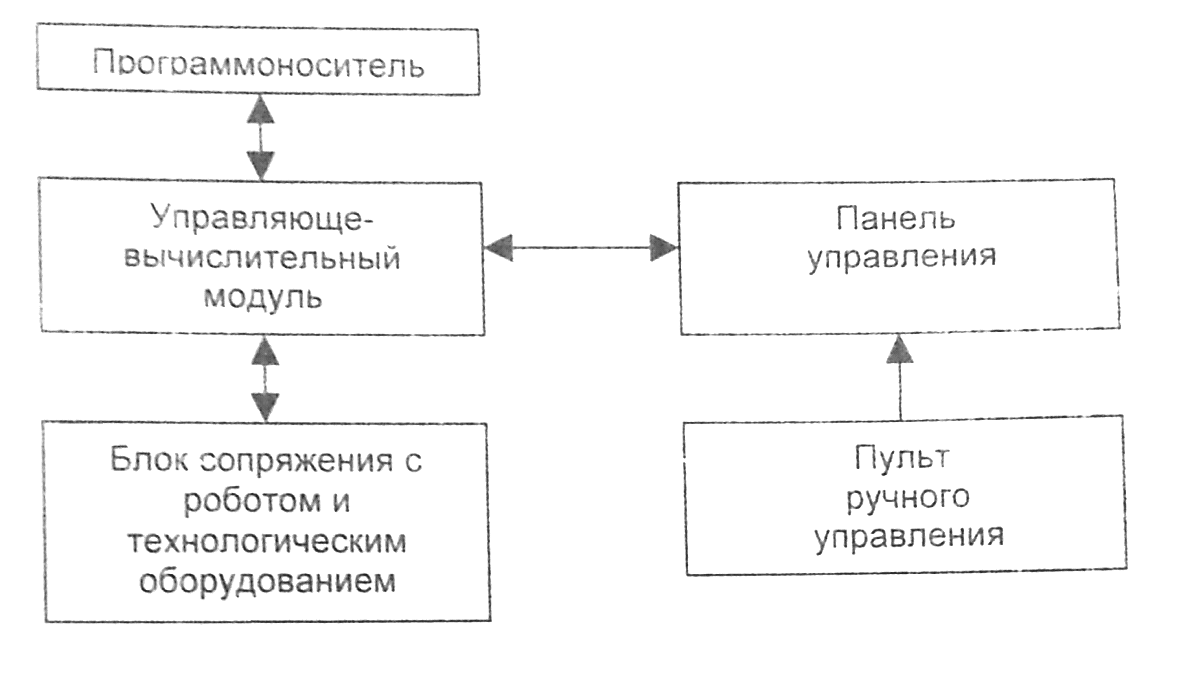
\includegraphics[width=.6\linewidth]{Figures/commonstructure.png}
    \caption{Обобщённая структура системы циклового управления}
    \label{fig:commonstructure}
\end{figure}

\subsection*{Промышленные роботы с цикловой системой управления}

В лабораторной работе рассматриваются три промышленных робота: МП-9С, МП-11 и 202М. Перечислим их основные исполнительные механизмы.

Система координат --- полярная. Датчики --- конечные регулируемые упоры, контакты электрические, магнитоуправляемые.

Степени подвижности манипуляторов:

\begin{itemize}
    \item МП-9С --- 3;
    \item МП-11 --- 4;
    \item РФ-202 --- 4.
\end{itemize}

Степени свободы манипуляторов:

\begin{itemize}
    \item МП-9C --- 4;
    \item МП-11 --- 6;
    \item РФ-202 --- 5.
\end{itemize}

\subsubsection*{МП-9С}

\begin{itemize}
    \item узел распределения воздуха;
    \item механизм подъема;
    \item механизм поворота;
    \item муфта с упорами;
    \item рука;
    \item амортизатор руки;
    \item амортизатор поворота;
    \item схват.
\end{itemize}

\subsubsection*{МП-11}

\begin{itemize}
    \item механизм подъема;
    \item механизм поворота;
    \item модуль поступательный (рука);
    \item демпфер руки;
    \item модуль поступательный (сдвиг схвата);
    \item модуль вращательный.
\end{itemize}

\subsubsection*{202М}

\begin{itemize}
    \item блок электроуправляемых клапанов (БЭК);
    \item модуль горизонтальных перемещений (МГП);
    \item модуль подъема МП-30;
    \item модуль поворота (МПВ);
    \item модуль ротации;
    \item механизм зажима (М3).
\end{itemize}

\subsection*{Выводы}

Ядром цикловой системы управления является управляюще-вычислительный модуль, формирующий микрооперации (управляющие импульсы) соответственно заданному алгоритму для выдачи их в операционные узлы и другие функциональные блоки.

Цикловое управление применяют в ПР, выполняющих вспомогательные операции по обслуживанию технологического оборудования при небольшом числе точек позиционирования манипуляторов по каждой степени подвижности (обычно около трех-четырех) и при сравнительно простых повторяющихся циклах движений \cite{oil:cycle}.

В лабораторной работе мы разобрали внутреннее устройство ЭЦПУ-6030, а также конструкцию и работу отдельных исполнительных механизмов промышленных роботов под управлением данной цикловой СУ.

\bibliography{../web.bib}

\clearpage
